\documentclass{article}

\usepackage[letterpaper,portrait,top=0.4in, left=0.6in, right=0.6in, bottom=1in]{geometry}

\usepackage{amsmath, amsfonts, amsthm, amssymb}
\usepackage{graphicx, float}
\usepackage{mathtools}
\usepackage{titlesec}
\usepackage{interval}
\usepackage{hyperref}
\usepackage{titling}
\usepackage{vwcol}
\usepackage{setspace}
\usepackage{empheq}
\usepackage{cancel}
\usepackage{esdiff}
\usepackage{multicol}
\usepackage{mdframed}
\usepackage{esdiff}
\usepackage{multicol}
\usepackage{tikz}

\intervalconfig {
	soft open fences
}

\newcommand{\alignedintertext}[1]{%
	\noalign{%
		\vskip\belowdisplayshortskip
		\vtop{\hsize=\linewidth#1\par
		\expandafter}%
		\expandafter\prevdepth\the\prevdepth
	}%
}

% \allowdisplaybreaks

%opening
\title{Problem Set \#47}
\author{Jayden Li}
\date{February 3, 2024}

\allowdisplaybreaks

\begin{document}
\setlength{\abovedisplayskip}{0pt}
\fontsize{12pt}{12pt}\selectfont
\maketitle

\section*{Problem 1}
\begin{itemize}
\item[(a)]
	Vertical:
	\begin{align*}
		\frac{(x-h)^2}{a^2}+\frac{(y-k)^2}{b^2}&=1 \\
		b^2(x-h)^2+a^2(y-k)^2&=a^2b^2 \\
		b^2\left(x^2-2hx+h^2\right)+a^2\left(y^2-2ky+k^2\right)&=a^2b^2 \\
		b^2x^2-2b^2hx+b^2h^2+a^2y^2-2a^2ky+a^2k^2-a^2b^2&=0 \\
		B^2-4AC&=(0)^2-4\left(b^2\right)\left(a^2\right) \\
		&=\boxed{-4a^2b^2}
	\end{align*}
	Horizontal:
	\begin{align*}
		\frac{(y-k)^2}{a^2}+\frac{(x-h)^2}{b^2}&=1 \\
		b^2(y-k)^2+a^2(x-h)^2&=a^2b^2 \\
		b^2\left(y^2-2ky+k^2\right)+a^2\left(x^2-2hx+h^2\right)&=a^2b^2 \\
		b^2y^2-2b^2ky+b^2k^2+a^2x^2-2a^2hx+a^2h^2-a^2b^2&=0 \\
		B^2-4AC&=(0)^2-4\left(a^2\right)\left(b^2\right) \\
		&=\boxed{-4a^2b^2}
	\end{align*}

\item[(b)]
	Vertical:
	\begin{align*}
		(x-h)^2&=4p(y-k) \\
		x^2-2hx+h^2&=4py-4pk \\
		x^2-2hx+(-4p)y+\left(h^2+4pk\right)&=0 \\
		B^2-4AC&=0-4(1)(0) \\
		&=\boxed{0}
	\end{align*}
	Horizontal:
	\begin{align*}
		(y-k)^2&=4p(x-h) \\
		y^2-2ky+k^2&=4px-4ph \\
		y^2-2ky+(-4p)x+\left(k^2+4ph\right)&=0 \\
		B^2-4AC&=0-4(0)(1) \\
		&=\boxed{0}
	\end{align*}

\item[(c)]
	Vertical:
	\begin{align*}
		\frac{(y-k)^2}{a^2}-\frac{(x-h)^2}{b^2}&=1 \\
		b^2(y-k)^2-a^2(x-h)^2&=a^2b^2 \\
		b^2\left(y^2-2ky+k^2\right)-a^2\left(x^2-2hx+h^2\right)-a^2b^2&=0 \\
		b^2y^2-2b^2ky+b^2k^2-a^2x^2+2a^2hx-a^2h^2-a^2b^2&=0 \\
		B^2-4AC&=0-4\left(-a^2\right)\left(b^2\right) \\
		&=\boxed{4a^2b^2}
	\end{align*}
	Horizontal:
	\begin{align*}
		\frac{(x-h)^2}{a^2}-\frac{(y-k)^2}{b^2}&=1 \\
		b^2(x-h)^2-a^2(y-k)^2&=a^2b^2 \\
		b^2\left(x^2-2hx+h^2\right)-a^2\left(y^2-2ky+k^2\right)-a^2b^2&=0 \\
		b^2x^2-2b^2hx+b^2h^2-a^2y^2+2a^2ky-a^2k^2-a^2b^2&=0 \\
		B^2-4AC&=0-4\left(b^2\right)\left(-a^2\right) \\
		&=\boxed{4a^2b^2}
	\end{align*}

\end{itemize}

Because $a,b\in\mathbb{R}^+$, I claim that the discriminant of an ellipse is negative, the discriminant of a parabola is 0, and the discriminant of a hyperbola is positive.

\section*{Problem 2}
\begin{itemize}
\item[(a)]
	\begin{align*}
		C_1:y^2+2y+12x+25&=0 \\
		B^2-4AC&=0-4(0)(1) \\
		&=0\;\boxed{\text{Parabola}} \\ \\
		C_2:x^2+2y^2-6x+4y+7&=0 \\
		B^2-4AC&=0-4(1)(2) \\
		&=-8\;\boxed{\text{Ellipse}} \\ \\
		C_3:2y^2-3x^2-4y+12x+8&=0 \\
		B^2-4AC&=0-4(-3)(2) \\
		&=12\;\boxed{\text{Hyperbola}}
	\end{align*}

\item[(b)]
	\begin{align*}
		C_1:y^2+2y+12x+25&=0 \\
		(y+1)^2-1+12x+25&=0 \\
		(y+1)^2&=-24-12x \\
		\Aboxed{(y+1)^2&=-12(x+2)} \\ \\
		C_2:x^2+2y^2-6x+4y+7&=0 \\
		(x-3)^2-9+2\left((y+1)^2-1\right)+7&=0 \\
		(x-3)^2+2(y+1)^2&=4 \\
		\Aboxed{\frac{(x-3)^2}{4}+\frac{(y+1)^2}{2}&=1} \\ \\
		C_3:2y^2-3x^2-4y+12x+8&=0 \\
		2\left((y-1)^2-1\right)-3\left((x-2)^2-4\right)+8&=0 \\
		2(y-1)^2-3(x-2)^2&=-18 \\
		3(x-2)^2-2(y-1)^2&=18 \\
		\Aboxed{\frac{(x-2)^2}{6}-\frac{(y-1)^2}{9}&=1}
	\end{align*}

\item[(c)]
	\phantom{}

	\centering
	\includegraphics*[width=\linewidth]{q2c.png}


\end{itemize}

\section*{Problem 3}
\begin{itemize}
\begin{minipage}[t]{0.4\linewidth}
	\item[(a)]
		\begin{align*}
			y^2&=16x \\
			2y\diff{y}{x}&=16 \\
			\diff{y}{x}&=\frac{8}{y} \\
			y-8a&=\frac{\cancel{8}}{\cancel{8}a}\left(x-4a^2\right) \\
			ay-8a^2&=x-4a^2 \\
			ay&=x+4a^2 \\
			\Aboxed{y&=\frac{x}{a}+4a}
		\end{align*}
		\qed
\end{minipage}
\begin{minipage}[t]{0.6\linewidth}
	\item[(b)]
		\phantom{}

		\hspace*{5pt}\includegraphics*[width=0.9\linewidth]{q3b.png}
\end{minipage}

\item[(c)]
The center is $(0,0)$ and $c=16/4=4$. The directrix is $x=0-c=-4$ and the focus is $F(4,0)$.

In part (a) we showed that the tangent line to the parabola at some point $P\left(4a^2,8a\right)$ is $y=\dfrac{x}{a}+4a$.
\begin{minipage}[t]{0.55\linewidth}
	The point $Q\left(-4,\dfrac{42}{5}\right)$ is also on this tangent line.
	\begin{align*}
		\frac{42}{5}&=\frac{-4}{a}+4a \\
		42a&=-20+20a^2 \\
		0&=10a^2-21a-10 \\
		a&=\frac{21\pm\sqrt{441+400}}{20} \\
		\intertext{We only consider the positive case because $a\geq0$.}
		a&=\frac{21+\sqrt{841}}{20} \\
		a&=\frac{21+29}{20} \\
		a&=\frac{5}{2}
	\end{align*}
	Thus we have $P\left(4\left(\dfrac{5}{2}\right)^2,8\left(\dfrac{5}{2}\right)\right)\implies P(25,20)$.
\end{minipage}
\begin{minipage}[t]{0.44\linewidth}
	\begin{align*}
		y&=\frac{x}{\frac{5}{2}}+4\left(\frac{5}{2}\right) \\
		y&=\frac{2x}{5}+10 \\
		\text{$x$-intercept}:0&=\frac{2x}{5}+10 \\
		2x&=-50 \\
		x&=-25 \implies S(-25,0)
	\end{align*}
\end{minipage}

\centering
\begin{minipage}{0.28\linewidth}
\begin{align*}
	S_{FSP}&=S_{SPD}-S_{FPD} \\
	S_{FSP}&=\frac{50\cdot20}{2}-\frac{21\cdot20}{2} \\
	S_{FSP}&=500-210 \\
	\Aboxed{S_{FSP}&=290} \\
\end{align*}
\end{minipage}
\begin{minipage}{0.7\linewidth}
	\vspace*{-50pt}
	\begin{tikzpicture}
		\path
			(0,0) coordinate (S) node[circle,fill,inner sep=1pt,label=below:${S(-25,0)}$](){}
			(4,0) coordinate (F) node[circle,fill,inner sep=1pt,label=below:${F(4,0)}$](){}
			(9,4) coordinate (P) node[circle,fill,inner sep=1pt,label=above:${P(25,20)}$](){}
			(9,0) coordinate (D) node[circle,fill,inner sep=1pt,label=below:${D(25,0)}$](){}
		;
		\draw
			(S) -- (F)
			(F) -- (P)
			(S) -- (P)
		;
		\draw[thick,dash dot]
			(D) -- (F)
			(D) -- (P)
		;
	\end{tikzpicture}
\end{minipage}
\end{itemize}

\section*{Problem 4}
\begin{itemize}
\item[(a)]
	\begin{minipage}[t]{0.49\linewidth}
		\begin{align*}
			x^2+4x+2y^2-14&=0 \\
			(x+2)^2-4+2y^2-14&=0 \\
			(x+2)^2+2y^2&=18 \\
			\frac{(x+2)^2}{18}+\frac{y^2}{9}&=1 \\
			\frac{(x+2)^2}{\left(3\sqrt{2}\right)^2}+\frac{y^2}{3^2}&=1
		\end{align*}
		Ellipse.

		\includegraphics*[width=0.9\linewidth]{q4a1.png}
	\end{minipage}
	\begin{minipage}[t]{0.49\linewidth}
		\begin{align*}
			9x^2-18x+16y^2-16&=0 \\
			9\left((x-1)^2-1\right)+16y^2-16&=0 \\
			9(x-1)^2+16y^2&=25 \\
			\frac{(x-1)^2}{\frac{25}{9}}+\frac{y^2}{\frac{25}{16}}&=1 \\
			\frac{(x-1)^2}{\left(\frac{5}{3}\right)^2}+\frac{y^2}{\left(\frac{5}{4}\right)^2}&=1
		\end{align*}
		Ellipse.

		\includegraphics*[width=0.85\linewidth]{q4a2.png}
	\end{minipage}

\item[(b)]
	\phantom{}
	
	\centering
	$\Bigg\{\begin{aligned}
		(x+2)^2+2y^2&=18 \\
		9(x-1)^2+16y^2&=25
	\end{aligned}$
	$\implies$
	$\Bigg\{\begin{aligned}
		16y^2&=144-8(x+2)^2 & (1) \\
		16y^2&=25-9(x-1)^2 & (2)
	\end{aligned}$
	\begin{align*}
		(1)-(2):0&=119-8(x+2)^2+9(x-1)^2 \\
		0&=119-8x^2-32x-32+9x^2-18x+9 \\
		0&=x^2-50x+96 \\
		0&=(x-2)(x-48) \\
		x&=2,x=-48
	\end{align*}
	\begin{minipage}[t]{0.4\linewidth}
		\begin{align*}
			(2+2)^2+2y^2&=18 \\
			2y^2&=2 \\
			y&=\pm1
		\end{align*}
		Intersections: \boxed{(2,1),(2,-1)}
	\end{minipage}
	\begin{minipage}[t]{0.4\linewidth}
		\begin{align*}
			(-48+2)^2+2y^2&=18 \\
			2y^2&=18-46^2
		\end{align*}
		No real solution for $y$.
	\end{minipage}
	\flushleft

\item[(c)]
	\begin{align*}
		(x-c)^2+y^2&=r^2 \\
		(2-c)^2+1^2&=r^2 \\
		4-4c+c^2+1&=r^2 \\
		c^2-4c+5&=r^2 \\
		\\
		(x-c)^2+y^2&=c^2-4c5 \\
		x^2-2xc+\cancel{c^2}+y^2&=\cancel{c^2}-4c+5 \\
		x^2-2xc+y^2&=5-4c
	\end{align*}
	\qed

\end{itemize}

\section*{Problem 6}
\begin{itemize}
\item[(a)]
	\begin{align*}
		\frac{x^2}{289}+\frac{y^2}{64}&=1 \\
		\frac{x^2}{17^2}+\frac{y^2}{8^2}&=1
	\end{align*}
	Horizontal, $h=0,k=0,a=17,b=8,c=\sqrt{289-64}=\sqrt{225}=15,e=\dfrac{c}{a}=\dfrac{15}{17}$, \boxed{\text{foci }(-15,0),(15,0)}, \boxed{\text{directrices }x=\pm\dfrac{a}{e}=\pm\dfrac{17}{\frac{15}{17}}=\pm\dfrac{289}{15}}
	
	\vspace*{15pt}
	\centering
	\includegraphics*[height=0.9\pagetotal-1in]{q6a.png}
	\flushleft

\item[(b)]
	Let $P(x_0,y_0)$ be a point. Because $PF$ where $F$ is the focus with positive $x$ coordinate, we have $F(15,0)$ and $x_0=15$. By the equation of the ellipse:

	\centering
	\begin{minipage}[t]{0.4\linewidth}
		\begin{align*}
			\frac{x_0^2}{289}+\frac{y_0^2}{64}&=1 \\
			\frac{225}{289}+\frac{y_0^2}{64}&=\frac{289}{289} \\
			\frac{y_0^2}{64}&=\frac{289-225}{289} \\
			y_0^2&=\frac{64^2}{17^2} \\
			y_0&=\pm\frac{64}{17}
		\end{align*}
	\end{minipage}
	\vline
	\begin{minipage}[t]{0.4\linewidth}
		\begin{align*}
			\frac{x^2}{289}+\frac{y^2}{64}&=1 \\
			\diff{}{x}\left[\frac{x^2}{289}\right]+\diff{}{x}\left[\frac{y^2}{64}\right]&=0 \\
			\frac{2x}{289}+\frac{y}{32}\diff{y}{x}&=0 \\
			\diff{y}{x}&=\frac{-\frac{2x}{289}}{\frac{y}{32}} \\
			\diff{y}{x}&=-\frac{64x}{289y}
		\end{align*}
	\end{minipage}
	\flushleft

	\begin{align*}
		\text{Tangent}:y-\left(\pm\frac{64}{17}\right)&=\left(-\frac{\cancel{64}(15)}{289\left(\pm\frac{\cancel{64}}{17}\right)}\right)\left(x-15\right) \\
		\text{$x$-intercept}:0-\left(\pm\frac{64}{17}\right)&=\mp\frac{15}{17}(x-15) \\
		\mp64&=\mp15(x-15) \\
		\mp64&=\mp15x\pm225 \\
		\mp(64+225)&=\mp15x \\
		\mp15x&=\mp289 \\
		x&=\pm\frac{289}{15}
	\end{align*}
	The $x$-intercepts of the tangent line at point $P$ is always at the directrix.
	
	\qed

\end{itemize}

\section*{Problem 7}
\begin{itemize}
\item[(a)]
	\begin{align*}
		\frac{x^2}{16}+\frac{y^2}{4}&=1 \\
		\diff{}{x}\left[\frac{x^2}{16}\right]+\diff{}{x}\left[\frac{y^2}{4}\right]&=0 \\
		\frac{x}{8}+\frac{y}{2}\diff{y}{x}&=0 \\
		\diff{y}{x}&=\frac{-\frac{x}{8}}{\frac{y}{2}} \\
		\diff{y}{x}&=-\frac{x}{4y}
	\end{align*}
	\begin{align*}
		\text{Normal line}:y-y_0&=\left(-\left(-\frac{x_0}{4y_0}\right)\right)^{-1}(x-x_0) \\
		y-2\sin\theta&=\frac{\cancel{4}\left(2\sin\theta\right)}{\cancel{4}\cos\theta}(x-4\cos\theta) \\
		y\cos\theta-2\sin\theta\cos\theta&=2\sin(\theta)\left(x-4\cos\theta\right) \\
		y\cos\theta-2\sin\theta\cos\theta&=2x\sin\theta-8\sin\theta\cos\theta \\
		2x\sin\theta-y\cos\theta&=6\sin\theta\cos\theta
	\end{align*}
	\qed

\item[(b)]
	We will find the $x$-intercept of the normal line at point $A$.
	\begin{align*}
		2x\sin\theta-\cancel{y\cos\theta}&=6\sin\theta\cos\theta \\
		x&=\frac{6\cancel{\sin\theta}\cos\theta}{2\cancel{\sin\theta}} \\
		x&=3\cos\theta
	\end{align*}

	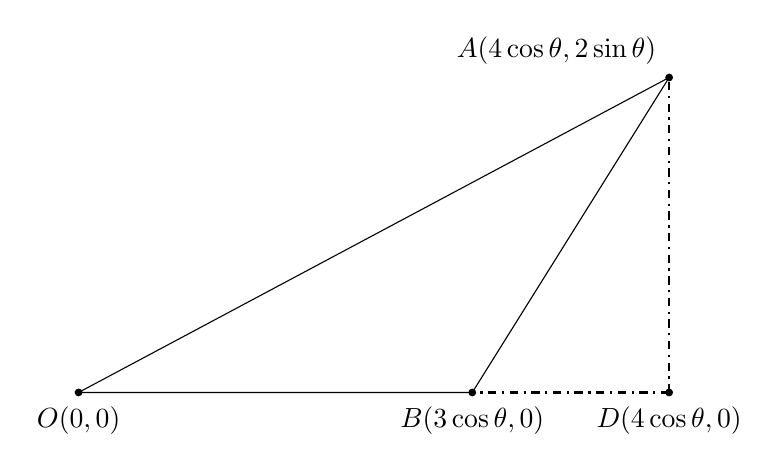
\begin{tikzpicture}[baseline=(current bounding box.north)]
		\path
			(0,0) coordinate (O) node[circle,fill,inner sep=1pt,label=below:${O(0,0)}$](){}
			(5,0) coordinate (B) node[circle,fill,inner sep=1pt,label=below:${B(3\cos\theta,0)}$](){}
			(7.5,4) coordinate (A) node[circle,fill,inner sep=1pt,label=above left:${A(4\cos\theta,2\sin\theta)}$](){}
			(7.5,0) coordinate (D) node[circle,fill,inner sep=1pt,label=below:${D(4\cos\theta,0)}$](){}
		;
		\draw
			(O) -- (B)
			(B) -- (A)
			(O) -- (A)
		;
		\draw[thick,dash dot]
			(D) -- (B)
			(D) -- (A)
		;
	\end{tikzpicture}
	\hfill
	\begin{minipage}[t]{0.5\linewidth}
		\begin{align*}
			S_{OAB}&=S_{OAD}-S_{ABD} \\
			S_{OAB}&=\frac{8\cos(\theta)\sin(\theta)}{2}-\frac{2\cos(\theta)\sin(\theta)}{2} \\
			S_{OAB}&=4\cos\theta\sin\theta-\cos\theta\sin\theta \\
			S_{OAB}&=\frac{3}{2}\left(2\cos\theta\sin\theta\right) \\
			S_{OAB}&=\frac{3}{2}\sin2\theta \\
			\Aboxed{\max S_{OAB}&=\frac{3}{2}} \\
		\end{align*}
	\end{minipage}


\end{itemize}

\end{document}